{
\usebackgroundtemplate{
 \tikz\node[opacity=0.1]{\includegraphics[width=1.1\paperwidth]{figures/TB-0067-300-00-A_stamp.pdf}};
 % \tikz\node[opacity=0.2]{\centering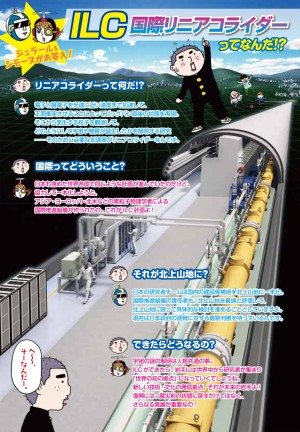
\includegraphics[height=\paperheight]{figures/Iwatecomics.jpg}};
 }
\begin{frame}{FLUKA simulation of the ILC Beam Dump}
\flukalogo
The beam is dumped into a water tank after collision.\\Neutrons ($\lesssim$\SI{e10}{\per\square\centi\metre\per\year}) are emitted that radiate the surroundings, and travel back towards the detectors.\\
\vspace*{0.1cm}
Redoing the simulation studies that were done in 2007 (design was not decided yet).
\begin{block}{Simulation step 1}
Simulating the neutrons from the beam dump with FLUKA, using the design drawings by B. Smith~\cite{Smith} to model the dump and the surrounding.
\end{block}

\begin{center}
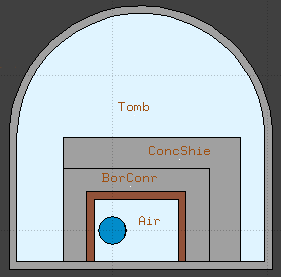
\includegraphics[height=0.35\textheight]{figures/Front_view_BeamDump_Tomb.png}
\hspace*{0.2cm}
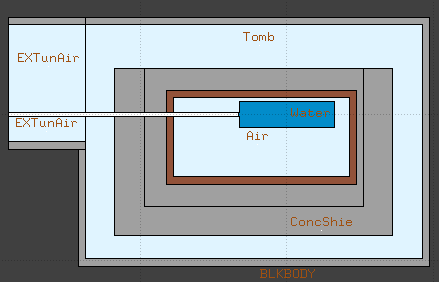
\includegraphics[height=0.35\textheight]{figures/Bird_view_BeamDump_Tomb.png}
\end{center}
\end{frame}

\begin{frame}{FLUKA simulation of the ILC Beam Dump}
\flukalogo
\begin{columns}
\begin{column}[c]{0.4\textwidth}
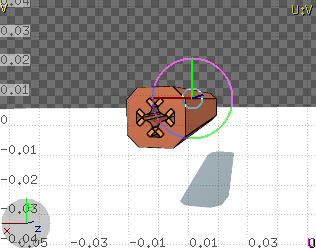
\includegraphics[height=0.45\textheight]{figures/FLUKA_quadrupole_model.png}\\
\small FLUKA simulation model of one of the ILC EXT lattice quadrupoles.
\end{column}
\begin{column}[c]{0.55\textwidth}
\begin{block}{Simulation step 2}
With Benno List (DESY): Python program to plug the real extraction line lattice into FLUKA.\\
Realistic simulation of the interaction between the neutrons and the lattice.
\end{block}
\begin{block}{Simulation step 3}
Simulating the neutrons reaching the interaction point in a full detector simulation.
\end{block}
\end{column}
\end{columns}
\end{frame}

\begin{frame}
 \flukalogo
 All goals of this study in an overview:
\begin{itemize}
 \item Simulating the neutron flux,
 \item the number of neutrons reaching the IP,
 \item the dosis of the surrounding,
 \item the influence of the water composition (amount of Deuterium),
 \item the effect of the beam dump design.
\end{itemize}
\vspace*{0.6cm}
\rule{12cm}{.1pt}
\begin{thebibliography}{9}
\setbeamertemplate{bibliography item}[text]
\bibitem{Smith} B. Smith (Rutherford Lab), \emph{Design drawings 0-TB-0067-300-00-A, 0-TB-0067-210-00-A, 0-TB-0067-404-00-A}, Dec. 2006 - Jan. 2007
\end{thebibliography}
\end{frame}
}

